\begin{frame}
\frametitle{Vector đơn vị}
\begin{tcolorbox}[colback=blue!10, colframe=blue!50!black, title=Định nghĩa]
    Một vector đơn vị là một vector có độ dài bằng 1. Ví dụ, nếu \(\mathbf{a}\) là một vector bất kỳ, thì vector đơn vị theo hướng của \(\mathbf{a}\) được tính bằng:
\begin{equation}
    \mathbf{u} = \frac{\mathbf{a}}{|\mathbf{a}|} 
\end{equation}
Vector này có độ dài bằng 1 và cùng hướng với \(\mathbf{a}\).
\end{tcolorbox}
\end{frame}

\begin{frame}
\frametitle{Cơ sở vector}
\begin{tcolorbox}[colback=blue!10, colframe=blue!50!black, title=Định nghĩa]
    Một vector cơ sở chuẩn hóa là một tập hợp các vector độc lập tuyến tính mà mọi vector trong không gian có thể được biểu diễn như một tổ hợp tuyến tính của các vector trong cơ sở đó.
\end{tcolorbox}
\end{frame}

\begin{frame}
\frametitle{Cơ sở vector}
\begin{columns}
\begin{column}{0.5\textwidth}
Trong không gian ba chiều, một vector cơ sở chuẩn hóa là tập hợp của ba vector đơn vị không đồng phẳng. Một vector có thể được xác định bằng cách biểu diễn nó dưới dạng tổ hợp tuyến tính của các vector đơn vị trong cơ sở.
\begin{equation}
    \mathbf{u}=a\mathbf{e}_1+b\mathbf{e}_2+c\mathbf{e}_3
\end{equation}
\end{column}
\begin{column}{0.5\textwidth}
\begin{figure}
\centering
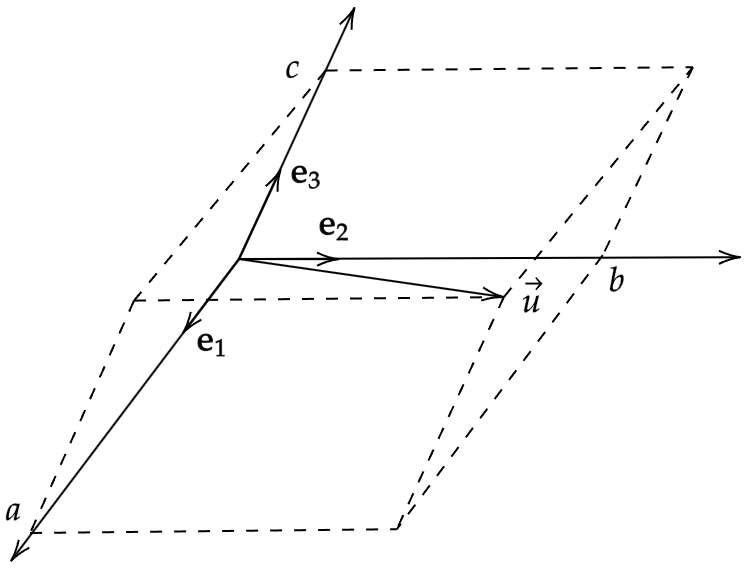
\includegraphics[width=0.9\textwidth]{Slides/Figure/cosovector.png}
\caption{Cơ sở \((\mathbf{e}_1, \mathbf{e}_2, \mathbf{e}_3)\)}
\end{figure}
\end{column}
\end{columns}
\end{frame}

\begin{frame}
\frametitle{Hệ tọa độ Descartes}
\begin{tcolorbox}[colback=blue!10, colframe=blue!50!black, title=Định nghĩa]
    Hệ tọa độ Descartes là một hệ tọa độ trực chuẩn, được xác định bởi một gốc tọa độ \(O\) và một vector cơ sở trực chuẩn (\(\mathbf{e}_1, \mathbf{e}_2, \mathbf{e}_3\)). Trong hệ tọa độ này, một điểm \(M\) trong không gian được xác định bởi ba tọa độ \((x, y, z)=(r_1, r_2, r_3)\),
    \begin{equation}
        \mathbf{r}=\mathbf{OM} = x\mathbf{e}_1 + y\mathbf{e}_2 + z\mathbf{e}_3.
    \end{equation}
\end{tcolorbox}
\end{frame}

\begin{frame}
\frametitle{Hệ tọa độ Descartes}
\begin{figure}
\centering
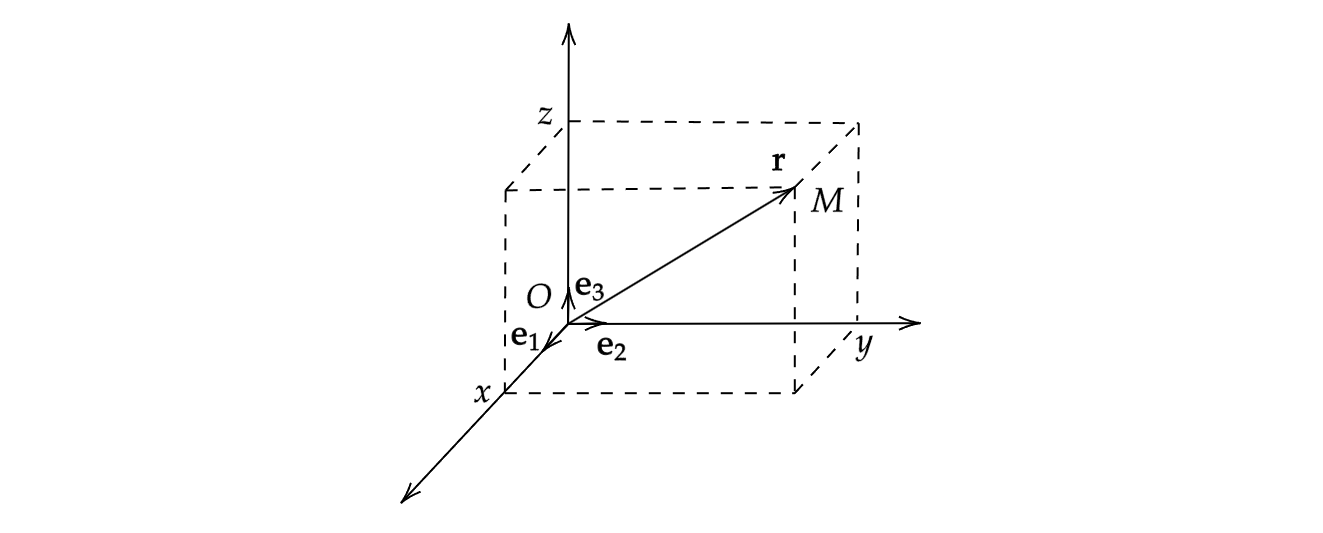
\includegraphics[width=1\textwidth]{Slides/Figure/toadodescartes.png}
\caption{Hệ tọa độ Descartes \(Oxyz\)}
\end{figure}
\end{frame}